\chapter{การทบทวนวรรณกรรมที่เกี่ยวข้อง}
\label{chapter:literature-review}

ในบทที่ 2 จะอธิบายถึงทฤษฎีที่เกี่ยวข้องในการสร้างแบบจำลองการระบุสายพันธุ์นก
ซึ่งประกอบด้วย ทฤษฎีเสียงและสัญญาณ (Sound and Signal) 
ทฤษฎีการประมวลผลภาพดิจิตัล (Digital Image Processing) ทฤษฎีการเรียนรู้ของเครื่อง (Machine Learning)
โครงข่ายประสาทเทียม (Artificial Neural Network) โครงข่ายประสาทเชิงลึก (Deep Neural Network) 
โครงข่ายประสาทแบบคอนโวลูชัน (Convolutional Neural Network, CNN) สถาปัตยกรรมต่าง ๆ ของโครงข่ายประสาทแบบคอนโวลูชันและการกำหนดองค์ประกอบ (CNN Architecture and Configuration)
เมตริกที่ใช้ในประเมินผลแบบจำลอง (Evaluation Metrics) และหลักการทำงานของเครื่องมือต่าง ๆ ที่ใช้ในงานวิจัย

\section{เสียงและสัญญาณ (Sound and Signal)}
เสียงเป็นพลังงานรูปแบบหนึ่งที่เกิดจากการสั่นสะเทือนของแหล่งกำเนิดเสียงผ่านตัวกลางและรับรู้ได้ด้วยหู ส่วนสัญญาณเป็นการแสดงถึงปริมาณที่แปรผันตามเวลา
ซึ่งมีคำจำกัดความที่ค่อนข้างเป็นนามธรรม และสัญญาณเสียงจะแสดงถึงความแปรปรวนของความกดอากาศเมื่อเวลาผ่านไป 
โดยมีไมโครโฟนที่ทำหน้าที่ในการวัดความแปรผันและสร้างสัญญาณไฟฟ้าที่เป็นตัวแทนของเสียง
และมีลำโพงที่ทำหน้าที่ในการรับสัญญาณไฟฟ้าและทำให้เกิดเสียง ซึ่งทั้งไมโครโฟนและลำโพงจะถูกเรียกว่า 
ทรานดิวเซอร์ (transducer) เนื่องจากทั้งไมโครโฟนและลำโพงเป็นอุปกรณ์ที่ทำหน้าที่รับพลังงานจากรูปแบบหนึ่ง
แล้วแปลงไปให้อยู่ในอีกรูปแบบหนึ่ง

\subsection{สัญญาณซ้ำคาบ (Periodic signals)}
เป็นลักษณะของสัญญาณที่มีรูปแบบการเกิดที่ซ้ำกันในหนึ่งช่วงเวลาที่เท่า ๆ กัน เรียกการวนครบรูปแบบของสัญญาณหนึ่งครั้งว่ารอบ (cycle) 
และเรียกระยะเวลาในแต่ละรอบว่าคาบ (period)  สัญญาณนี้จะมีลักษณะคล้ายกับกราฟของฟังก์ชันไซน์ ดังภาพ~\ref{Fig:Sine_wave}

\begin{figure}[h]
    \centering
    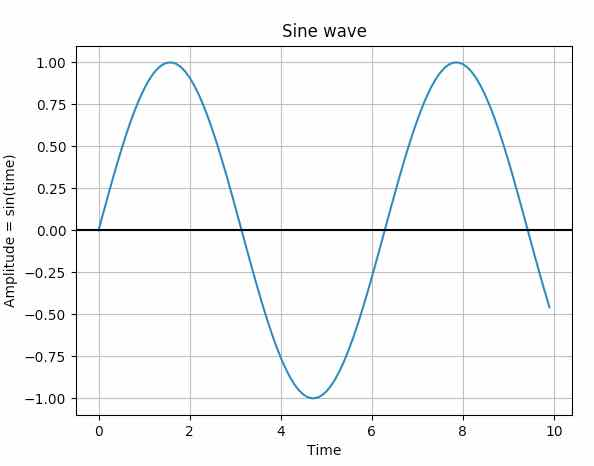
\includegraphics[scale = 0.3]{sinewave.jpg}
    \caption{แสดงกราฟของฟังก์ชันไซน์}
    \label{Fig:Sine_wave}
\end{figure}

ความถี่ของสัญญาณมีหน่วยเป็นจำนวนของรอบต่อวินาที ซึ่งเป็นค่าที่ตรงกันข้ามกับคาบ ซึ่งมีหน่วยคือ รอบต่อวินาที หรือ เฮิรตซ์ (Hz) 
ในเครื่องดนตรีส่วนใหญ่จะให้สัญญาณซ้ำคาบเพียงแต่ไม่ได้อยู่ในรูปแบบของสัญญาณไซน์ (sinusoidal) 
ตัวอย่างเช่นสัญญาณของเสียงไวโอลิน

\begin{figure}[h]
    \centering
    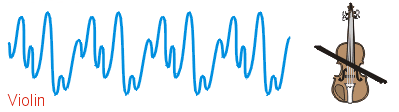
\includegraphics[scale = 0.5]{violin_waveform.png}
    \caption{แสดงสัญญาณซ้ำคาบ}
    \label{Fig:Periodic_signal}
\end{figure}
% \begin{figure}[h]
%     \includegraphics[]{}
%     \caption{}
%     \label{}
% \end{figure}

เราเรียกรูปร่างของสัญญาณซ้ำคาบเหล่านี้ว่า รูปแบบของคลื่น (waveform) เครื่องดนตรีส่วนใหญ่จะสร้างรูปแบบของคลื่นที่ซับซ้อนมากกว่าสัญญาณไซน์ 
รูปแบบของคลื่นจะเป็นเครื่องกำหนดลักษณะของเสียงร้องหรือเสียงดนตรี ดังภาพ~\ref{Fig:Periodic_signal} ซึ่งเป็นการรับรู้เกี่ยวกับคุณภาพของเสียง 
และมนุษย์มักจะรับรู้เสียงที่มีความซับซ้อนมากกว่ารูปแบบคลื่นของไซน์ 

\subsection{สัญญาไม่ซ้ำคาบ (Non-periodic signals)}
เป็นสัญญานที่มีการเปลี่ยนแปลงที่ไม่สามารถระบุรูปแบบที่แน่นอนของสัญญาณได้ เช่นเสียงการพูดคุยของมนุษย์ 
สัญญาณเหล่านี้สามารถมองเห็นได้โดยการนำเสนอในรูปแบบของเสปกโตรแกรม (spectrograms)

\subsection{การสุ่มตัวอย่าง (Sampling)}
การสุ่มตัวอย่างคือการเปลี่ยนแปลงสัญญาณที่มีความต่อเนื่องทางเวลา (Continuos signal) ให้อยู่ในรูปแบบที่ไม่ต่อเนื่องทางเวลา (Discrete signal) ด้วยการสุ่มเก็บตัวอย่างของสัญญาณ
ในช่วงเวลาที่ห่างเท่า ๆ กัน ซึ่งช่วงเวลาดังกล่าวจะถูกเรียกว่า อัตราสุ่มสัญญาณ (Sampling rate) ในการสุ่มสัญญาณจำเป็นต้องเลือกอัตราการสุ่มให้เหมาะสมกับความถี่ของสัญญาณนั้น ๆ
เนื่องจากในเวลาที่ต้องการแปลงสัญญาณกลับไปเป็นสัญญาณที่มีความต่อเนื่องทางเวลาจะได้สัญญาณต้นฉบับที่ถูกต้องและครบถ้วน~\cite{AT1987}

\subsection{สเปกโตรแกรม (Spectrograms)}
สเปกโตรแกรมเป็นภาพหรือแผนภาพของสเปกตรัม(Spectrum) โดยที่สเปกตรัมเป็นแถบคลื่นความถี่ของเสียงที่รวมกับแสงที่มนุษย์สามารถมองเห็นได้ 
โดยสเปกโตรแกรมทำให้สามารถมองเห็นผลลัพธ์ของการแบ่งเสียงออกเป็นส่วน ๆ ได้ โดยเรียกการเปลี่ยนของเสียงในแต่ละส่วนละส่วนเป็นสเปกโตรแกรมนี้จะถูกเรียกว่า Short-Time Fourier Transform (STFT)
โดยที่แกน x ของสเปกโตรแกรมจะแสดงเวลาและแสดงความถีบนแกน y โดยในแต่ละคอลัมน์จะแสดงสเปกตรัมของส่วนนั้น ๆ โดยใช้สีในการแสดงแอมพลิจูด (Amplitude) หรือความเข้มของเสียงนั้น

\begin{figure}[h]
    \centering
    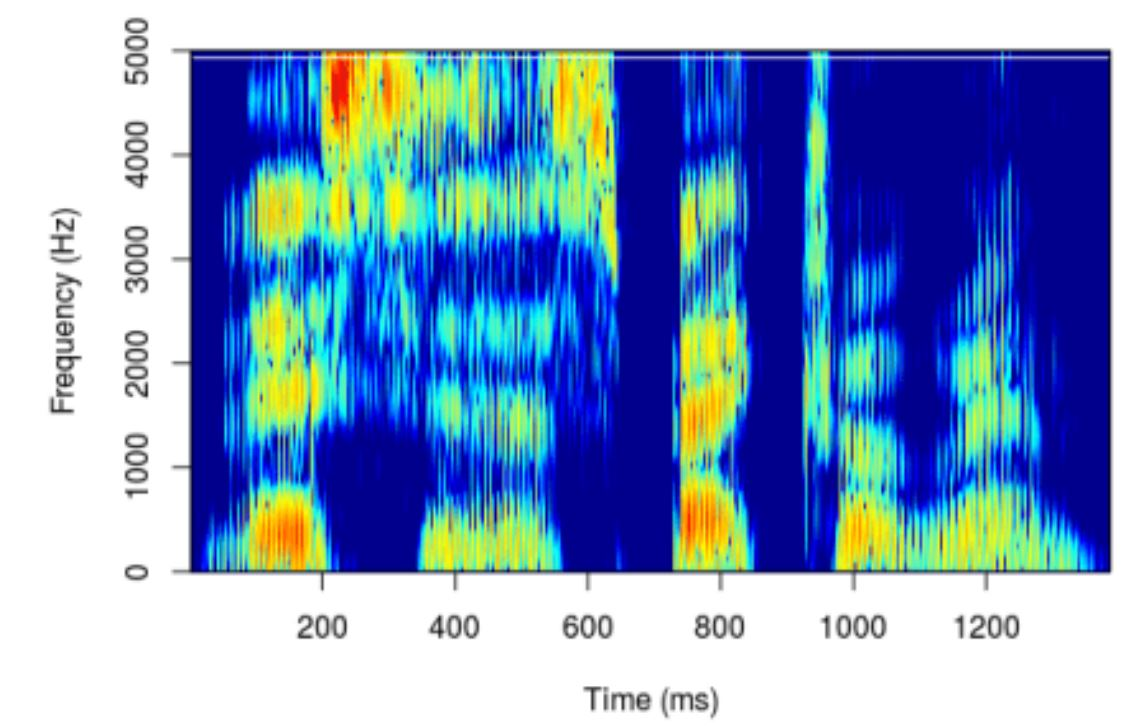
\includegraphics[scale = 0.4]{spectogram_1.JPG}
    \caption{แสดงตัวอย่างภาพสเปกโตรแกรม}
    \label{Fig:specto_gram_1}
\end{figure}

\subsection{สัญญาณรบกวน (Noise)}
เป็นเสียงหรือสัญญาณที่ไม่พึงประสงค์ที่อาจเกิดจากการทำงานผิดพลาดของอุปกรณ์ที่ใช้ในการเก็บข้อมูล หรือสร้างขึ้นเพื่อศึกษาลักษณะ รูปแบบ และทำความเข้าใจกับสัญญาณรบกวนเหล่านี้ได้
โดยสัญญาณรบกวนที่สร้างง่ายที่สุดถูกเรียกว่า เสียงสัญญาณรบกวนที่ไม่เกี่ยวข้องกันแบบสม่ำเสมอ (Uncorrelated Uniform Noise) หรือ UU Noise โดยที่ Uniform หมายถึงสัญญาณจะมีการสุ่มค่าจากการกระจายที่สม่ำเสมอ 
นั่นคือทุก ๆ ค่าในช่วงนั้นมีโอกาสที่จะเท่ากัน และ uncorrelated ที่หมายถึงไม่เกี่ยวข้องกันหรือเป็นอิสระต่อกัน กล่าวคือการรู้ค่าเพียงค่าเดียวไม่สามารถให้ข้อมูลอื่น ๆ ได้
และมี 3 สิ่งที่ควรทราบเกี่ยวกับสัญญาณรบกวนและสเปกตรัมคือ 1. การกระจายของสัญญาณสุ่ม 2. ความสัมพันธ์ของแต่ละค่าในสัญญาณเป็นอิสระจากกันหรือไม่ 
และ 3. ความสัมพันธ์ระหว่างกำลัง (Power) กับความถี่ จากสามสิ่งที่ควรทราบนี้จะสามารถสร้างสัญญาณรบกวนได้ 3 ลักษณะคือ สัญญาณรบกวนบราวน์ (Brownian noise) 
หรือสัญญาณรบกวนสีแดง (Red noise) สัญญาณรบกวนสีชมพู (Pink Noise) และ Gaussian Noise หรือสัญญาณรบกวนสีขาว สัญญาณรบกวนโดยปกติจะถูกสังเคราะห์ขึ้นจากสมการ~\ref{eq:noise_generate}

\begin{equation}
    P = \frac{K}{f^{\beta}}
    \label{eq:noise_generate}
\end{equation}

โดยที่ $P$ คือกำลัง $f$ เป็นค่าของความถี่และ $K$ คือจุดตัดของเส้นตรง จากสมการข้างต้นเราสามารถทราบความสัมพันธ์ระหว่างกำลังและความถี่ของสัญญาณรบกวนต่าง ๆ ได้ คือเมื่อ
$P = K / f^{2}$ ผลลัพธ์ของสัญญาณรบกวนนี้จะตกอยู่ในช่วงของสเปกตรัมแสงสีแดง ซึ่งมีความถี่ที่ต่ำที่สุด ในขณะที่ถ้าเราเปลี่ยนค่าของ $\beta$ ให้เท่ากับ 0 สัญญาณรบกวนที่เกิดขึ้นจะตกอยู่ในช่วงของสเปกตรัมแสงสีขาว 
ทำให้เกิดเป็นสัญญาณรบกวนสีขาว และเมื่อค่า $\beta$ มีค่าอยู่ในระหว่าง 0 ถึง 2 ผลลัพธ์ของสัญญาณรบกวนจะอยู่ระหว่างช่วงสเปกตรัมแสงสีขาวและสีแดง จึงเรียกสัญญาณรบกวณที่อยู่ในช่วงนี้ว่าสัญญาณณบกวนสีชมพู

\section{ทฤษฎีการประมวลผลภาพดิจิตัล (Digital Image Processing)}

\section{การเรียนรู้ของเครื่อง (Machine Learning)}
การเรียนรู้ของเครื่องคือการที่คอมพิวเตอร์สามารถที่จะเรียนรู้ได้ด้วยตัวเอง โดยที่ไม่ต้องเขียนโปรแกรมสั่งให้คอมพิวเตอร์ทำงาน 
ซึ่งจะแตกต่างกับการเขียนโปรแกรมในสมัยก่อน ซึ่งในสมัยก่อนโปรแกรมเมอร์ต้องทำการโปรแกรมไปยังคอมพิวเตอร์เพือให้ได้ผลลัพธ์ออกมา 
แต่ในการเรียนรู้ของเครื่องผู้ใช้งานเพียงแค่ใส่ข้อมูลและระบุผลลัพธ์ที่ต้องการเท่านั้น 
คอมพิวเตอร์จะทำการเรียนรู้ด้วยตนเองแล้วแสดงผลลัพธ์ที่ได้ออกมาเป็นโปรแกรมที่สามารถนำไปใช้ในการทำนายผลลัพธ์ของข้อมูลได้ดังรูป~\ref{Fig:tradition_vs_ml}

\begin{figure}[h]
    \centering
    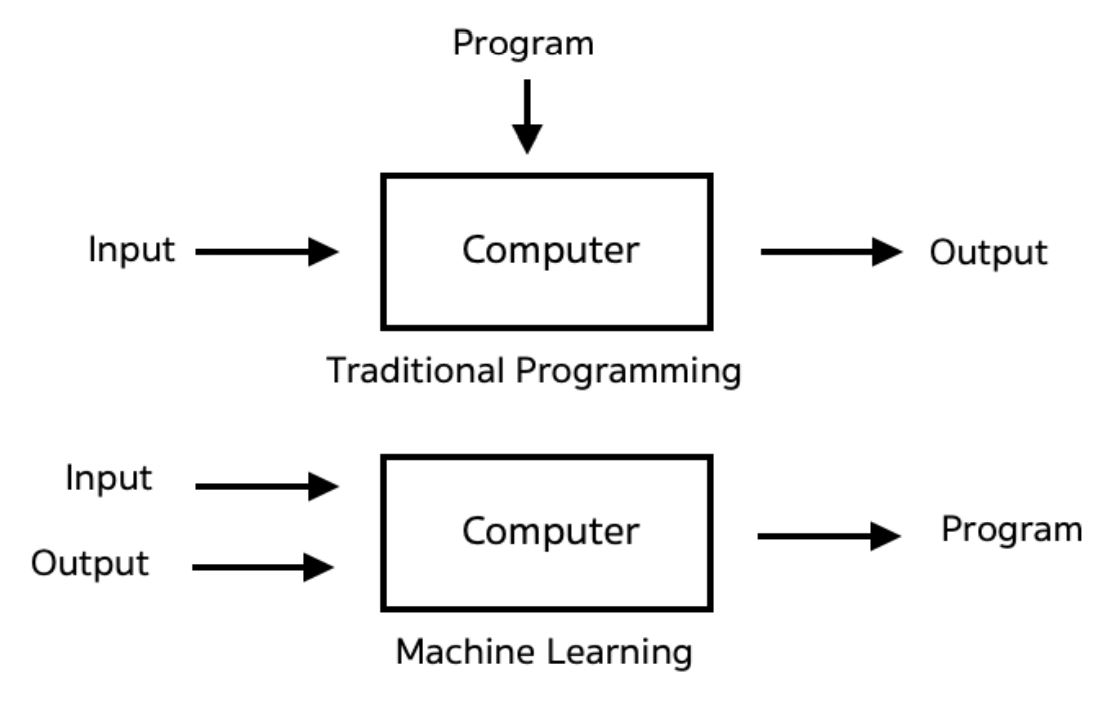
\includegraphics[scale = 0.4]{tradition_v_ml.JPG}
    \caption{แสดงความแตกต่างระหว่างการเขียนโปรแกรมในอดีตกับการเรียนรู้ของเครื่อง}
    \label{Fig:tradition_vs_ml}
\end{figure}
\FloatBarrier

โดยการเรียนรู้ของเครื่องนั้นจะประกอบไปด้วยข้อมูลและเครื่องมือทางสถิติที่ใช้ในการทำนายผลลัพธ์หรือหารูปแบบของข้อมูลที่เข้าไป
เครื่องจะทำการเรียนรู้ที่มีลักษณะคล้ายกันกับมนุษย์คือเรียนรู้จากประสบการณ์ 
ยิ่งมีประสบการณ์มากก็จะยิ่งมีความเชี่ยวชาญมากทำให้ง่ายต่อการทำนายผลลัพธ์ที่เกิดขึ้นจากสถานการณ์ที่คล้าย ๆ กันได้
และเพื่อเพิ่มความแม่นยำในการทำนายผลลัพธ์ เครื่อง (Machine) ก็ควรจะมีการฝึกด้วยข้อมูลจำนวนที่มากเพียงพอ 
ที่เครื่องจะสามารถค้นพบผลลัพธ์ผ่านรูปแบบหรือแบบแผนที่ซ้ำ ๆ กันได้ และการเรียนรู้ของเครื่องนั้นสามารถแบ่งรูปแบบการเรียนรู้ได้เป็น 2 ลักษณะใหญ่ ๆ คือ

\subsection{การเรียนรู้แบบมีผู้สอน (Supervised Learning)}
การเรียนรู้แบบมีผู้สอนคือการที่คอมพิวเตอร์สามารถหาผลลัพธ์ของข้อมูลได้ดัวยตัวเองหลังจากที่มีการเรียนรู้จากชุดข้อมูลตัวอย่างไปแล้วระยะเวลาหนึ่ง 
โดยเริ่มต้นโปรแกรมเมอร์จะเขียนโปรแกรมให้คอมพิวเตอร์สร้างแบบจำลอง (Model) 
ขึ้นมาจากชุดข้อมูลและผลลัพธ์ตัวอย่าง โดยที่ถ้าชุดข้อมูลตัวอย่างมีความหลากหลายและมีจำนวนมากอาจทำให้ผลลัพธ์ที่ได้จากการเรียนรู้นั้นมีความแม่นยำมากขึ้น 
กระบวนการนี้จะถูกเรียกว่าการฝึกอบรม(Train) เมื่อผลลัพธ์ที่ได้มีความแม่นยำมากขึ้น 
จะกล่าวได้ว่าแบบจำลองที่ได้จากการฝึกอบรมนี้มีความสามารถในการทำนายผลลัพธ์ได้ถูกต้องมากขึ้น 
การเรียนรู้แบบมีผู้สอนสามารถแบ่งออกเป็นประเภทย่อยได้อีก 2 ประเภทย่อยคือ

\begin{itemize}
    \item\textbf{การแยกประเภท (Classification)}\par
    แบบจำลองการแยกประเภทเป็นแบบจำลองที่ใช้ในการแบ่งข้อมูลออกเป็นกลุ่ม 
    โดยข้อมูลที่นำมาใช้ต้องมีกลุ่มเป้าหมายของข้อมูลกำกับอยู่ด้วย 
    และคอมพิวเตอร์จะเรียนรู้จากลักษณะของข้อมูลที่ใส่เข้ามา 
    เช่นการทำนายว่าลูกค้าอยู่ในกลุ่มลูกค้าชั้นดีหรือลูกค้าชั้นแย่ จากข้อมูลต่าง ๆ ของลูกค้าเช่น เพศ, อายุ, เงินเดือนเป็นต้น

    \item\textbf{การทำนายผลข้อมูล (Regression)}\par
    แบบจำลองการทำนายผลข้อมูลจะทำการคำนวณผลลัพธ์ของข้อมูลด้วยปัจจัยต่าง ๆ ที่เกี่ยวข้องกับผลลัพธ์ 
    เช่น การทำนายราคาที่ดินจากทำเลที่ตั้ง, ขนาดของที่ดิน, สาธารณูปโภค 
    และหลักฐานการรับรองสิทธิ์เป็นต้น\par
    ความแตกต่างระหว่างการแยกประเภทกับการทำนายผลข้อมูลคือ 
    การแยกประเภทจะให้ผลลัพธ์เป็นข้อมูลที่ไม่ต่อเนื่องมีลักษณะเป็นกลุ่ม 
    เช่น หมวดหมู่ ใช่หรือไม่ใช่ และระดับความเสี่ยงเป็นต้น ในขณะที่การทำนายผลข้อมูลจะให้ผลลัพธ์เป็นข้อมูลแบบต่อเนื่อง เช่น 
    ตัวเลขที่ได้จากการคำนวณของแบบจำลองที่มีค่าระหว่าง 0 ถึง 100 เป็นต้น
\end{itemize}

\subsection{การเรียนรู้แบบไม่มีผู้สอน (Unsupervised Learning)}
การเรียนรู้แบบไม่มีผู้สอนคือการที่คอมพิวเตอร์สามารถเรียนรู้ได้ด้วยตัวเองจากข้อมูลที่ใส่เข้าไป 
โดยข้อมูลนั้นไม่จำเป็นต้องมีผลลัพธ์กำกับไว้ ประเภทหลักๆของการเรียนรู้แบบไม่มีผู้สอนคือ การแบ่งกลุ่มข้อมูล (Clustering)

\begin{itemize}
    \item\textbf{การแบ่งกลุ่มข้อมูล (Clustering)}\par
    การแบ่งกลุ่มข้อมูลคือการที่คอมพิวเตอร์สามารถที่จะแบ่งข้อมูลออกเป็นกลุ่ม ๆ ได้ด้วยตัวเอง 
    โดยที่ข้อมูลที่มีลักษณะใกล้เคียงกันจะอยู่ในกลุ่มเดียวกัน และข้อมูลที่ต่างกันจะอยู่คนละกลุ่มกัน 
    เช่น การจัดกลุ่มของลูกค้าจากพฤติกรรมการซื้อสินค้าของลูกค้า โดยที่ถ้าลูกค้ามีลักษณะการซื้อสินค้าที่คล้ายกันจะถูกจัดอยู่ในกลุ่มเดียวกัน 
    และลูกค้าที่มีลักษณะการซื้อสินค้าต่างกันจะอยู่คนละกลุ่มกัน\par
    ปัจจุบันการเรียนรู้ของเครื่องได้ถูกนำไปประยุกต์ใช้อย่างแพร่หลายเช่น 
    การคัดแยกจดหมายอิเล็กทรอนิกส์ การตรวจจับใบหน้าของมนุษย์ 
    และการทำให้รถสามารถเคลื่อนที่ได้โดยไร้คนขับ
\end{itemize}




\section{โครงข่ายประสาทเทียม (Artificial Neural Network)}
โครงข่ายประสาทเทียมเป็นการจำลองระบบประสาทของสิ่งมีชีวิตขึ้นมา เพื่อให้คอมพิวเตอร์สามารถคำนวณผลลัพธ์ออกมาได้ จะประกอบไปด้วยชั้น (Layer) ต่าง ๆ 3 
ชั้นที่สำคัญคือ ชั้นขาเข้า (Input Layer) ชั้นซ่อน (Hidden Layer) 
และสุดท้ายคือชั้นผลลัพธ์ขาออก (Output Layer) เมื่อมีชุดข้อมูลเข้ามาที่ชั้นขาเข้า 
ชุดข้อมูลนี้จะถูกประมวลผลในชั้นซ่อน และนำเสนอผลลัพธ์ที่ได้ผ่านชั้นผลลัพธ์ขาออก 
นอกจากนี้ยังสามารถอธิบายการทำงานของโครงข่ายประสาทเทียมผ่านฟังก์ชันทางคณิตศาสตร์ได้ \par

\begin{figure}[h]
    \centering
    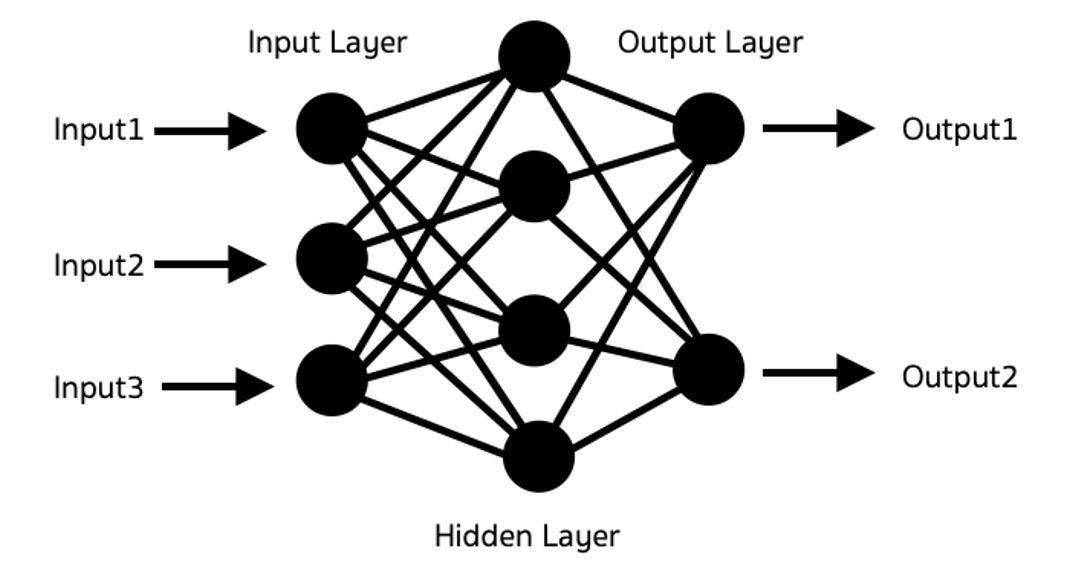
\includegraphics[scale = 0.4]{artificial example.JPG}
    \caption{แสดงโครงสร้างของโครงข่ายประสาทเทียม}
    \label{Fig:artificial_example}
\end{figure}

การหาค่าผิดพลาด (Error) ของโครงข่ายประสาทเทียมจะใช้อัลกอรึทึมที่ชื่อว่า feed-forward neural networks 
คือข้อมูลจะถูกส่งไปข้างหน้าเพียงหนึ่งทิศทางเท่านั้น 
กล่าวคือข้อมูลจะถูกส่งจากชั้นขาเข้าไปยังชั้นซ่อนและส่งต่อไปยังชั้นผลลัพธ์ขาออกเท่านั้นและเมื่อได้ผลลัพธ์ออกมาแล้ว 
จะนำผลลัพธ์ที่ได้มาคำนวณกับค่าเป้าหมายเพื่อหาค่าผิดพลาด 
จากนั้นนำค่าผิดพลาดที่คำนวณได้ไปใช้ในการปรับค่าน้ำหนักของข้อมูล \par

ข้อมูลที่รับเข้ามาจะถูกคูณด้วยค่าน้ำหนัก (Weight) ก่อนจะถูกส่งต่อไปยังเซลล์ประสาทในชั้นซ่อน 
โดยในหนึ่งเซลล์ประสาทในชั้นซ่อนนั้นจะประกอบไปด้วยฟังก์ชันทางคณิตศาสตร์หรือ Activation function 
ที่ใช้ในการพิจารณาผลลัพธ์ดังภาพ~\ref{Fig:Activation_function}

\begin{figure}[h]
    \centering
    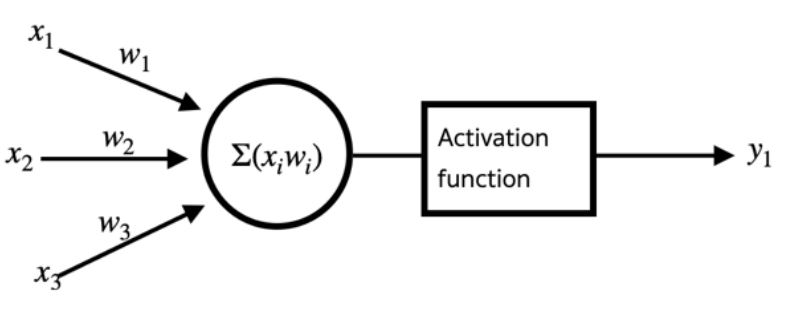
\includegraphics[scale = 0.5]{activation_function.JPG}
    \caption{แสดงการทำงานของเซลล์ประสาทเทียมกับ Activation Function}
    \label{Fig:Activation_function}
\end{figure}

ซึ่ง Activation function ที่เป็นที่นิยมได้แก่ Sigmoid, Softmax และ ReLU Activation Function โดยที่ 
Sigmoid Function จะเป็นการเปลี่ยนผลรวมของข้อมูลที่เข้ามาให้มีค่าอยู่ระหว่าง 0 ถึง 1 เท่านั้น จึงเหมาะที่จะถูกนำไปใช้ในงานที่ต้องการ ผลลัพธ์ หรือ output
ที่เป็นความน่าจะเป็น (Probability) ส่วน Softmax Function จะให้ผลลัพธ์เป็น 0 ถึง 1 เหมือนกันแต่สามารถนำไปใช้งานได้หลากหลายกว่า
เพราะเป็นการแสดงผลลัพธ์ของหลาย ๆ ข้อมูลที่เข้ามารวมกันเป็นหลาย ๆ ผลลัพธ์ซึ่งเหมาะมากกับการนำไปใช้ในการจำแนกประเภทหลายคลาส (Multi-Class Classification) 
ส่วน ReLU Function คือฟังก์ชั่นที่ได้รับความนิยมสูงสุดในขณะนี้ โดยที่ถ้าได้ผลลัพธ์ต่ำกว่า 0 จะได้ผลลัพธ์เป็น 0 โดยทันที
แต่หากได้ค่ามากกว่าหรือเท่ากับ 0 ก็จะได้ผลลัพธ์เป็นค่านั้น ๆ ซึ่ง ReLU นั้นนิยมใช้มากในงานโครงข่ายประสาทแบบคอนโวลูชันและโครงข่ายประสาทเชิงลึก \par

\begin{figure}[h]
    \centering
    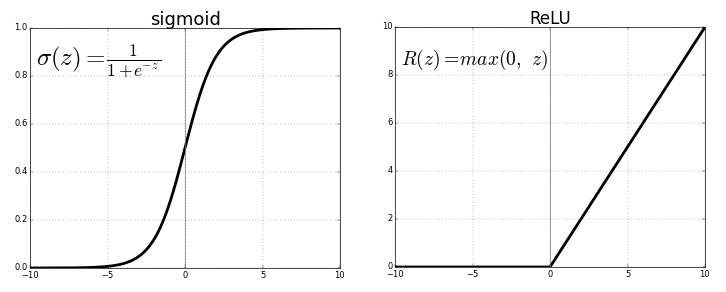
\includegraphics[scale = 0.4]{sigmoin_v_relu.png}
    \caption{รูปเปรียบเทียบระหว่าง Sigmoid และ ReLU Function}
    \label{Fig:Sigmoind_v_Relu}
\end{figure}

\subsection{โครงข่ายประสาทเชิงลึก (Deep Neural Network)} \par
โครงข่ายประสาทเชิงลึกเป็นการต่อยอดมาจากโครงข่ายประสาทเทียม (Artificial Neural Network) และเป็นส่วนหนึ่งที่อยู่ภายใต้ศาสตร์การเรียนรู้ของเครื่อง (Machine Learning)
กล่าวคือในชั้นซ่อนของโครงข่ายประสาทเชิงลึกจะมีจำนวนมากกว่าจำนวนชั้นซ่อนของโครงข่ายประสาทเทียม
และใช้อัลกอริทึมในการปรับค่าน้ำหนักที่ต่างกันด้วย

\begin{figure}[h]
    \centering
    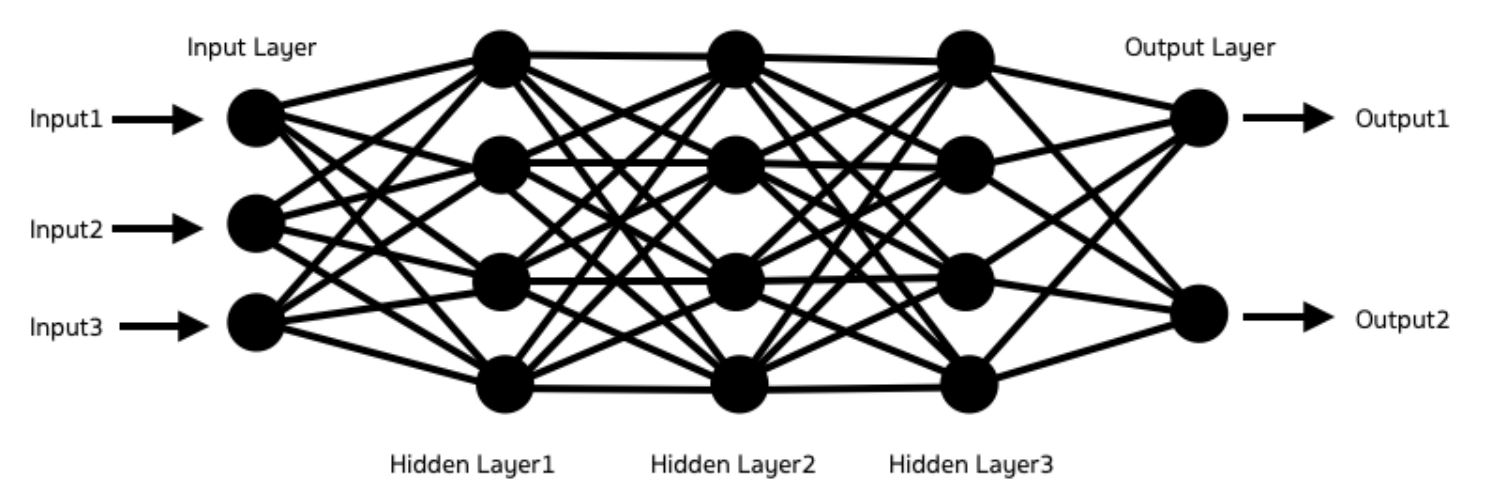
\includegraphics[scale = 0.4]{Deep_neural_ex.JPG}
    \caption{แสดงโครงสร้างของโครงข่ายประสาทเชิงลึก}
    \label{Fig:Deep_neuralnet}
\end{figure}

ในโครงข่ายประสาทเทียมเชิงลึกจะใช้อัลกอริทึม Backward Propagation ในการปรับค่าน้ำหนัก 
ในขั้นแรกจะทำ feed-forward เมื่อเสร็จสิ้นแล้วจะทําการปรับค่าน้ำหนักของโครงข่ายประสาทเทียมเชิงลึกโดยใช้จะใช้อัลกอริทึม 
Backward Propagation และใช้อัลกอริทึม Gradient Descent ในการหาค่าน้ำหนักที่เหมาะสมที่สุด

\begin{itemize}

    \item\textbf{การส่งค่าย้อนกลับ (Backward Propagation or Back Propagation)}

    ก่อนที่จะมีการส่งค่าย้อนกลับนั้น ต้องทำการคำนวณหาค่าผิดพลาด (Error) จากผลลัพธ์ที่ได้มาจากโครงข่ายประสาทเทียมก่อน 
    โดยนําผลลัพธ์ที่ได้จากโครงข่ายประสาทเทียมมาเปรียบเทียบกับผลลัพธ์เป้าหมาย 
    เมื่อได้ค่าผิดพลาดมาแล้วจะทำการส่งค่าผิดพลาดนี้กลับไปยังพารามิเตอร์ที่มีส่วนเกี่ยวข้องหรือก็คือค่าของน้ำหนักนั่นเอง
    เนื่องจากค่าผลลัพธ์ที่ได้จากโครงข่ายประสาทเทียมนั้น ถูกคำนวณมาจากค่าของน้ำหนัก สิ่งที่เราต้องทราบคือค่าน้ำหนักแต่ละตัวนั้นมี
    ผลกระทบต่อค่าผิดพลาดมากน้อยแค่ไหน โดยคำนวณจากการหาอนุพันธ์ของค่าผิดพลาดเทียบกับน้ำหนัก

    \begin{figure}[h]
        \centering
        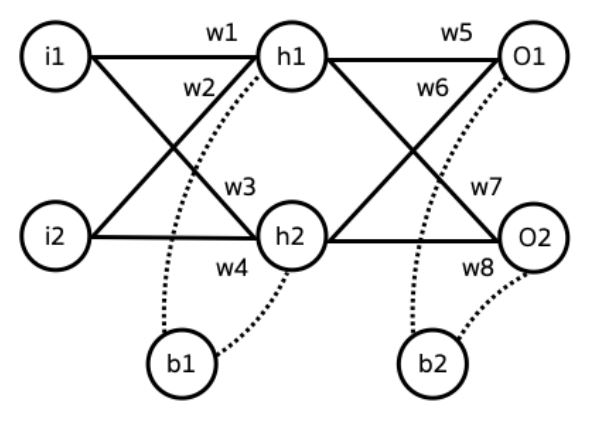
\includegraphics[scale = 0.5]{artificial example_2.JPG}
        \caption{แสดงโครงข่ายประสาทเทียม}
        \label{Fig:Artificial_2}
    \end{figure}

    เพื่อให้ง่ายต่อการอธิบายจึงยกตัวอย่างของโครงข่ายประสาทเทียมดังภาพ~\ref{Fig:Artificial_2} มาช่วยในการอธิบาย
    โดยเซลล์ i คือเซลล์ประสาทเทียมในชั้นขาเข้า เซลล์ h แทนเซลล์ประสาทเทียมในชั้นซ่อน และเซลล์
    O แทนเซล์ประสาทเทียมในชั้นผลลัพธ์ โดยผลลัพธ์ที่ได้จากโครงข่ายประสาทเทียมนี้จะสามารถคํานวณได้ตามสมการตัวอย่าง

    \begin{equation}
        \centering
        O1 = h1 \cdot w_5 + h2 \cdot + w_6 + b_2
        \label{eq:arti_ex_1}
    \end{equation}

    จากสมการ~\ref{eq:arti_ex_1} ทำให้ทราบว่าผลลัพธ์ที่ได้จากเซลล์ผลลัพธ์จะเท่ากับ
    ผลลัพธ์ของเซลล์ในชั้นซ่อนก่อนหน้าคูณด้วยน้ำหนักแล้วบวกด้วยค่าอคติหรือ bias 
    ในทำนองเดียวกันการหาผลลัพธ์ของเซลล์ในชั้นซ่อนจะหาจากค่าของข้อมูลในชั้นขาเข้าคูณด้วยน้ำหนักและบวกด้วยค่าอคติดังสมการ~\ref{eq:arti_ex_2}

    \begin{equation}
        \centering
        h1 = i1 \cdot w_1 + i2 \cdot + w_2 + b_1
        \label{eq:arti_ex_2}
    \end{equation}

    หลังจากที่ทราบค่าในแต่ละเซลล์ผลลัพธ์ O1 และ O2 แล้วจะทำการหาผลรวมของค่าผิดพลาด (Error) จากสมการ~\ref{eq:sum_error}

    \begin{equation}
        \centering
        E_{total} = \sum_{i=1}^{n}\frac{1}{2}(y_{i} - f(x_i))^2
        \label{eq:sum_error}
    \end{equation}

    จากสมการแสดงการคำนวณค่าผิดพลาด โดยที่ $y_{target}$ คือผลลัพธ์เป้าหมายและ $y_{out}$ คือผลลัพธ์ที่ได้จากโครงข่ายประสาทเทียม 
    โดยที่เอาค่าที่ได้จากเซลล์ O1 ไปคำนวณด้วย Activation function แล้วนำมาเปรียบเทียบกับผลลัพธ์เป้าหมาย หลังจากที่ได้ค่าผลรวมความผิดพลาดมาแล้ว 
    เราจะทำการหาอนุพันธ์ของค่าผิดพลาดเทียบกับน้ำหนักทีละตัว เพื่อให้ได้ค่าเกรเดียน (Gradient) ของน้ำหนักเพื่อนำไปใช้ในการปรับน้ำหนักดังสมการ~\ref{eq:gradient_1}

    \begin{equation}
        \centering
        \frac{\partial Error(w)}{\partial W}
        \label{eq:gradient_1}
    \end{equation}

    โดยที่ $E_{total}$ คือผลรวมของค่าความผิดพลาด และ $w_i$ คือน้ำหนักตัวที่ $i$
    และเนื่องจากสมการ~\ref{eq:gradient_1}เป็นสมการเชิงอนุพันธ์ย่อย (Partial Differential) จึงต้องใช้กฎลูกโซ่ (Chain Rule) 
    เข้ามาช่วยในการคำนวณ ตัวอย่างเช่นสมการต่อไปนี้ีจะแสดงการหาอนุพันธ์ระหว่างผลรวมของค่าผิดพลาดกับค่าน้ำหนักตัวที่ 5 ($w5$)

    \begin{equation}
        \centering
        \frac{\partial E_{total}}{\partial w_5} = \frac{\partial E_{total}}{\partial y_{out1}} x \frac{y_{out1}}{\partial O_1} x \frac{\partial O_1}{\partial w_5}
        \label{eq:Error_total_1}
    \end{equation}

    หลังจากที่คำนวณสมการข้างต้นแล้ว จะได้ค่าของเกรเดียนของน้ำหนักตัวที่ 5 หรืออัตราการเปลี่ยนแปลงของน้ำหนักตัวที่
    5 หลังจากนั้นเราจะนำค่าเกรเดียนที่ได้ไปใช้ในการปรับค่า
    น้ำหนักเพื่อที่จะลดค่าผิดพลาดให้มีค่าน้อยที่สุด โดยใช้สมการดังนี้

    \begin{equation}
        \centering
        W_{new} = W_{old} - \alpha *\frac{\partial Error(w)}{\partial W}
        \label{eq:new_weight_1}
    \end{equation}

    โดยที่ $\alpha$ คือค่าอัตราการเรียนรู้ (Learning Rate) เป็นค่าไฮเปอร์พารามิเตอร์ (Hyperparameter) ที่ควบคุมการปรับค่าน้ำหนักของ
    โครงข่ายประสาทเทียมว่ามากหรือน้อยแค่ไหนในหนึ่งขั้นตอน (Step) ของการฝึกอบรมแบบจำลอง ซึ่งเป็นค่าคงที่ 
    และหลังจากทำการปรับน้ำหนักแล้ว จะเริ่มทำการคำนวณแบบเดียวกันกับค่าน้ำหนักตัวอื่น ๆ ในชั้นเดียวกันจนครบทุกตัว ขั้นต่อไปคือการคำนวณในทำนาองเดียวกันกับชั้นก่อนหน้า
    โดยที่จะคำนวณอย่างนี้ซ้ำ ไปจนกระทั่งน้ำหนักทุกตัวได้รับการปรับปรุงจนหมด

\end{itemize}


\subsection{โครงข่ายประสาทแบบคอนโวลูชัน (Convolutional Neural Network, CNN)}
โครงข่ายประสาทแบบคอนโวลูชันเป็นโครงข่ายประสาทเทียมหนึ่งในกลุ่มของ bio-inspired โดยจะจำลองการมองเห็นของมนุษย์ที่จะมองพื้นที่เป็นย่อย ๆ และนำพื้นที่ย่อย ๆ มารวมกันเพื่อดูว่าสิ่งที่มนุษย์มองอยู่นั้นคืออะไร
ซึ่งในการมองพื้นที่ย่อย ๆ ของมนุษย์นั้น จะมีการคัดแยกคุณลักษณะ (Feature Extraction) ของพื้นที่นั้น ๆ เช่นลายเส้น สี การรวมกันของลายเส้นและสี
การมองภาพผ่านดวงตาของมนุษย์นั้นจะแบ่งการมองออกเป็นสองจุดใหญ่ ๆ คือจุดที่โฟกัสหรือสนใจและบริเวณต่าง ๆ โดยรอบของจุดนั้น ๆ  เมื่อนำมาประกอบกันจะทำให้สมองประมวลผลสิ่งที่เห็นและจะทำให้ทราบว่าสิ่ง ๆ นั้นคืออะไร

\begin{figure}[h]
    \centering
    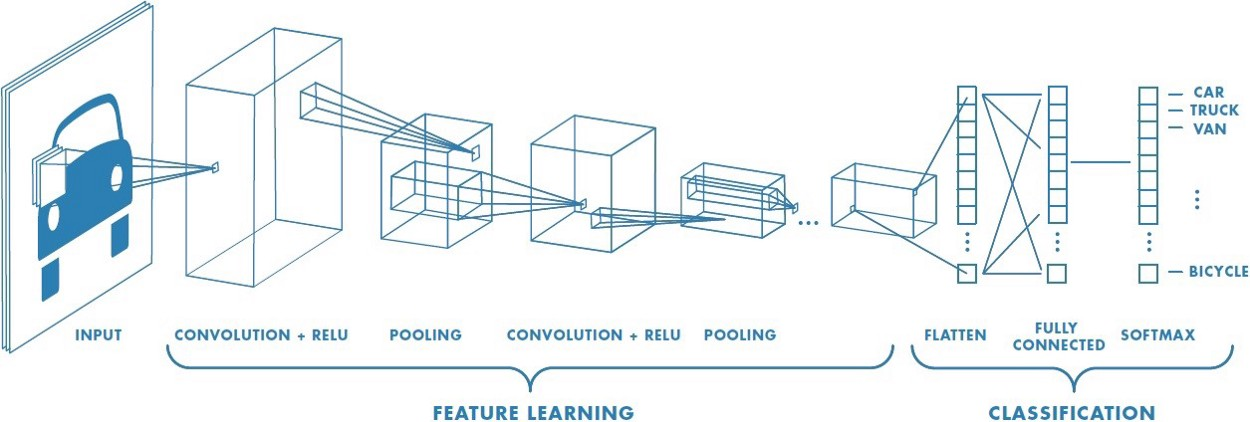
\includegraphics[scale = 0.3]{cnn_1.jpeg}
    \caption{แสดงสถาปัตยกรรมของโครงข่ายประสาทเทียมแบบคอนโวลูชัน}
    \label{Fig:conv_arch_ex1}
\end{figure}

\begin{itemize}

    \item \textbf{การคัดแยกคุณลักษณะเด่น (Feature Extraction) ในโครงข่ายประสาทแบบคอนโวลูชัน} \par
    
    เพื่อให้โครงข่ายประสาทเทียมมีการคำนวณที่สอดคล้องกับแนวคิดของตัวมันเองนั้น 
    จึงมีการนำคณิตศาสตร์เข้ามาช่วยในการคำนวณโดยใช้หลักการเดียวกับ คอนโวลูชันเชิงพื้นที่ (Spatial Convolution) 
    ในงานด้านการประมวลผลภาพดิจิตัล (Digital Image Processing) การคำนวณนี้จะมีการกำหนดค่าของตัวกรอง (Filter) ที่จะช่วยในการดึงคุณลักษณะที่ใช้ในการเรียนรู้และจดจำวัตถุออกมา
    โดยปกติตัวกรองหนึ่งตัวจะดึงคุณลักษณะที่สนใจออกมาได้เพียงหนึ่งคุณลักษณะเท่านั้น ทำให้จำเป็นต้องมีตัวกรองหลายตัวเพื่อหาคุณลักษณะทางพื้นที่หลาย ๆ อย่างมาประกอบกัน
    
    \item \textbf{ลักษณะของตัวกรอง} \par
    
    ตัวกรองสำหรับภาพดิจิตัลนั้นโดยทั่วไปจะเป็นตาราง 2 มิติที่มีขนาดภาพตามพื้นที่ย่อย ๆ ที่ต้องพิจารณา

    \begin{figure}[h]
        \centering
        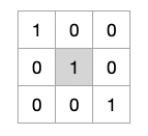
\includegraphics[scale = 0.5]{filter_3x3.JPG}
        \caption{แสดงตัวกรองขนาด 3 X 3}
        \label{Fig:filter_3X3}
    \end{figure}

    โดยที่ช่องที่แรเงาตรงกลางจะถูกเรียกว่า Anchor มีหน้าที่เอาไว้ทาบกับพิกเซลของข้อมูลภาพขาเข้า 
    เริ่มแรกตัวกรองจะถูกวางทาบลงไปบนพิกเซลแรกของข้อมูลภาพ และหลังจากนั้นจะถูกเลื่อนไปในตำแหน่งของพิกเซลถัดไปทีละพิกเซลจนครบทุกพิกเซลในภาพ
    ในขั้นตอนนี้มีข้อจำกัดคือ ตัวกรองจะไม่สามารถถูกนำไปทาบกับพิกเซลที่อยู่ใกล้กับขอบภาพได้ เนื่องจากตัวกรองจะเกินออกไปนอกภาพ เมื่อตัวกรองถูกเลื่อนไปจนครบทุกตำแหน่งที่สามารถเลื่อนไปได้แล้ว สิ่งที่ได้จากขั้นตอนนี้ จะถูกเรียกว่า 
    ผังคุณลักษณะ (Feature Map)

    \item \textbf{การทำคอนโวลูชัน} \par
    
    การทำคอนโวลูชันเป็นการคูณเมทริกซ์ระหว่างข้อมูลภาพขาเข้า กับตัวกรอง เมื่อนำตัวกรองไทาบลงบนข้อมูลภาพขาเข้าแล้ว ค่าในทุก ๆ 
    ตำแหน่งที่ตรงกันจะทำการคูณกัน หลังจากนั้นจะรวมผลลัพธ์ที่ได้ทั้งหมดเข้าด้วยกันในตำแหน่งที่เรียกว่า Anchor หลังจากนั้นจะเลื่อนตัวกรองไปยังตำแหน่งถัดไป 
    เมื่อทำครบทุกพิกเซลแล้วจะได้ผลลัพธ์ที่เป็นผังคุณลักษณะออกมา
    
    \begin{figure}[h]
        \centering
        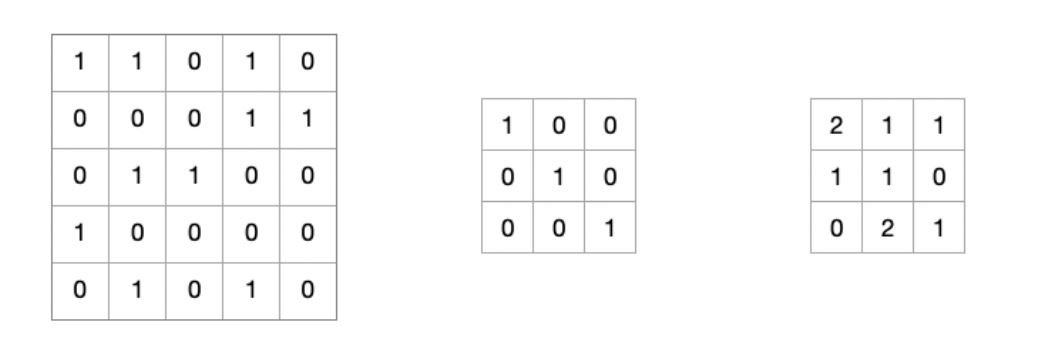
\includegraphics[scale = 0.4]{feature_mapre_1.JPG}
        \caption{แสดงตัวอย่างของข้อมูลภาพขาเข้า ตัวกรอง และผังคุณลักษณะ}
        \label{Fig:input_fil_feature}
    \end{figure}

    \begin{figure}[h]
        \centering
        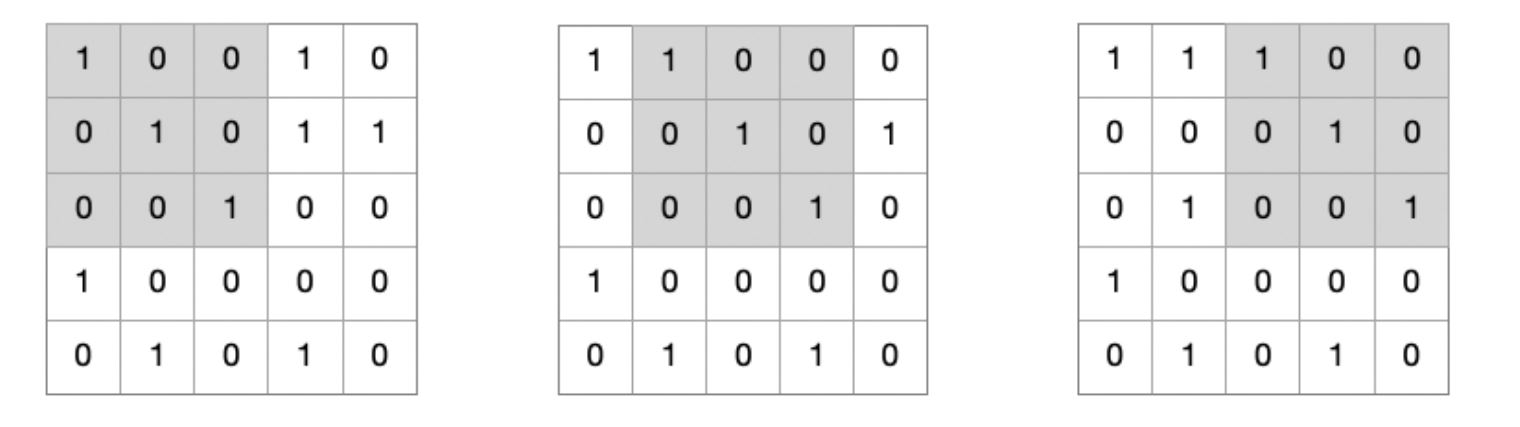
\includegraphics[scale = 0.35]{feature_mapre_2.JPG}
        \caption{แสดงตัวอย่างลักษณะการเคลื่อนที่ของตัวกรองเพื่อให้ได้ผลลัพธ์ดังภาพ~\ref{Fig:input_fil_feature}}
        \label{Fig:feature_stride_eg_1}
    \end{figure}
    
    \item \textbf{Stride และ Padding} \par
    
    \textbf{Stride} เปรียบเสมือนระยะห่างในการเลื่อนพิกเซลของตัวกรอง Stride สามารถกำหนดให้มากขึ้นได้ 
    ถ้าต้องการคำนวณหาคุณลักษณะที่มีพื้นที่ทับซ้อนกันน้อยลง แต่ในขณะเดียวกันเมื่อค่า Stride มากขึ้นผังคุณลักษณะจะมีขนาดเล็กลง

    \begin{figure}[h]
        \centering
        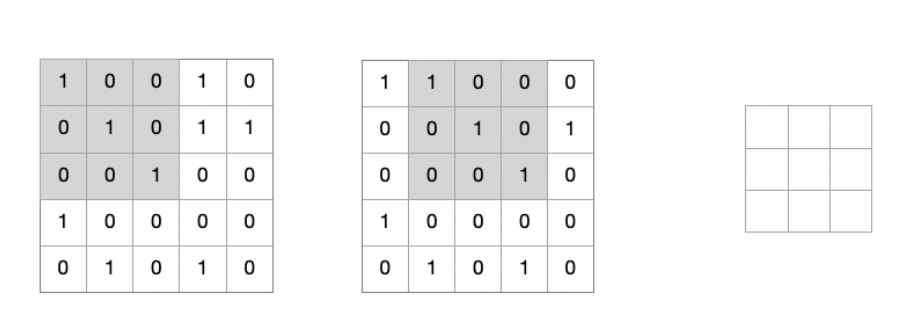
\includegraphics[scale = 0.5]{feature_mapre_3.JPG}
        \caption{แสดงการเคลื่อนที่ของตัวกรองเมื่อ Stride มีค่าเท่ากับ 1 และแสดงผลลัพธ์ของผังคุณลักษณะที่ได้}
        \label{Fig:feature_stride_eg_2}
    \end{figure}
    \begin{figure}[h]
        \centering
        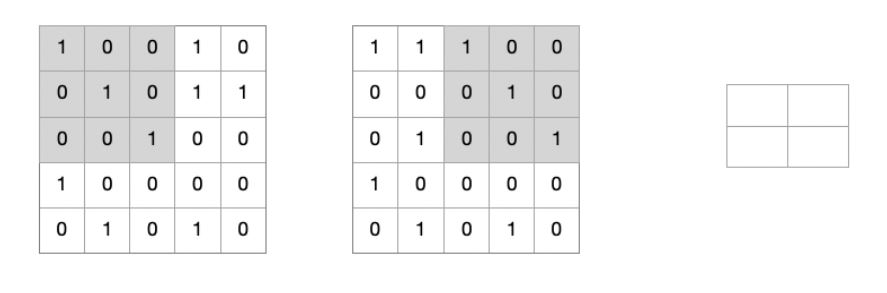
\includegraphics[scale = 0.5]{feature_mapre_4.JPG}
        \caption{แสดงการเคลื่อนที่ของตัวกรองเมื่อ Stride มีค่าเท่ากับ 2 และแสดงผลลัพธ์ของผังคุณลักษณะที่ได้}
        \label{Fig:feature_stride_eg_3}
    \end{figure}
    \FloatBarrier

    \textbf{Padding} จากขั้นตอนการทำคอนโวลูชันที่ผ่านมาจะเห็นได้ว่าผังคุณลักษณะจะมีขนาดเล็กลงกว่าข้อมูลภาพขาเข้า 
    หากต้องการให้ผังคุณลักษณะมีขนาดเท่ากับข้อมูลภาพขาเข้าก็จะต้องมีการเติม 0 หรือค่าต่าง ๆ เข้าไปรอบ ๆ ข้อมูลภาพขาเข้า 
    วิธีนี้จะช่วยแก้ปัญหาในกรณีที่ขอบของภาพมีความสำคัญที่ส่งผลต่อการตัดสินใจดังรูป~\ref{Fig:padding_1}

    \begin{figure}[h]
        \centering
        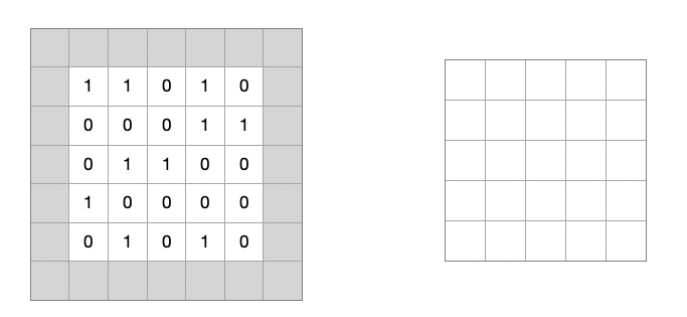
\includegraphics[scale = 0.45]{padding_1.JPG}
        \caption{แสดงข้อมูลรูปภาพที่มีการทำ Padding และแสดงของผังคุณลักษณะที่ได้หลังจากการทำ Padding}
        \label{Fig:padding_1}
    \end{figure}
    
    \item \textbf{Max Pooling} \par
    มนุษย์เราจำแนกวัตถุโดยอาศัยการดูรายละเอียดเล็ก ๆ และมองแบบคร่าว ๆ บนพื้นที่ใหญ่ ๆ จึงทำให้เกิดปัญหาหากต้องใช้ข้อมูลที่หยาบหรือละเอียดอย่างใดอย่างหนึ่งในการจำแนกวัตถุ
    ดังนั้นในการฝึกอบรมแบบจำลองควรมีข้อมูลทั้งหยาบและละเอียดควบคู่กันไป 
    เพื่อให้สามารถจัดการกับปัญหานี้ได้ การย่อขนาดภาพจึงเป็นสิ่งสำคัญ 
    เนื่องจากขนาดของตัวกรองมีความเท่าเดิมอยู่ตลอด 
    ถ้าข้อมูลภาพที่เข้ามามีขนาดใหญ่เราจะได้ข้อมูลที่มีความละเอียดมาก 
    ในขณะเดียวกันถ้าข้อมูลภาพมีขนาดเล็กลง ด้วยตัวกรองขนาดเท่าเดิม
    ตัวกรองจะสามารถครอบคลุมพื้นที่ของวัตถุเดิมได้มากขึ้น Pooling 
    คือความสามารถในการย่อรูปแบบหนึ่งมี 2 ประเภทหลัก ๆ ที่เป็นที่นิยมคือ Max Pooling 
    และ Mean Pooling โดย Max Pooling 
    จะนำค่าที่มากที่สุดที่ตัวกรองทาบทับ อยู่มาเป็นผลลัพธ์ โดยตัวกรองของ Max Pooling 
    จะทำงานในลักษณะเดียวกันกับ ตัวกรองในการทําคอนโวลูชัน โดยทั่วไปในการทํา Max Pooling 
    จะใช้ตัวกรองขนาด 2 x 2 และมี Stride เท่ากับ 2

    \begin{figure}[h]
        \centering
        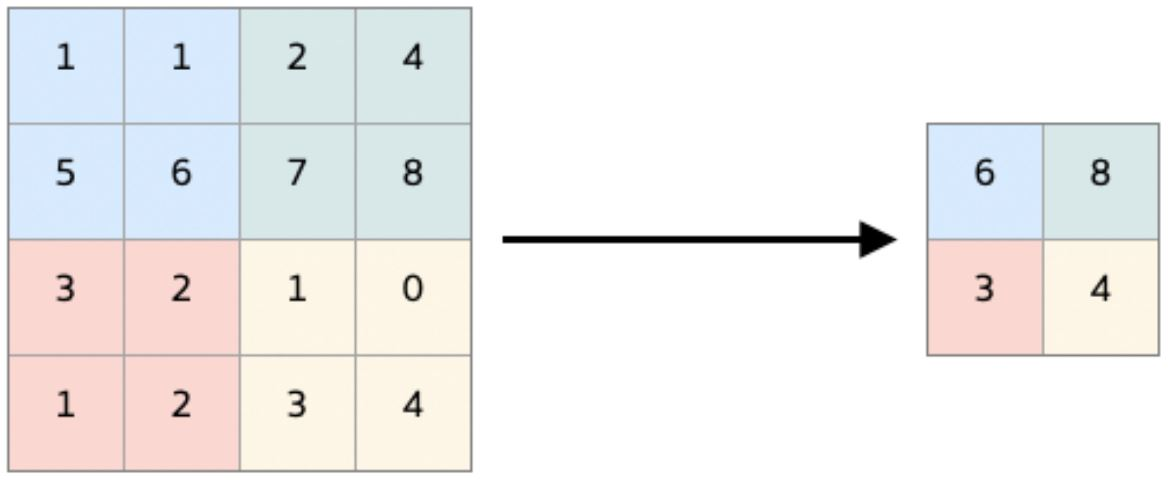
\includegraphics[scale = 0.3]{max_pool_1.JPG}
        \caption{แสดงการทำ Max Pooling ที่มีขนาดตัวกรองเท่ากับ 2 x 2 และ stride เท่ากับ 2}
        \label{Fig:max_pool_1}
    \end{figure}
    
\end{itemize}

\section{สถาปัตยกรรมต่าง ๆ ของโครงข่ายประสาทแบบคอนโวลูชันและการกำหนดองค์ประกอบ (CNN Architecture and Configuration)}


\section{เมตริกที่ใช้ในประเมินผลแบบจำลอง (Evaluation Metrics)}
เมตริกที่ใช้ในการประเมินผลแบบจำลอง โดยปกติแล้วจะมีให้เลือกใช้หลายวิธีด้วยกัน แต่การจะหยิบเมตริกมาใช้ในการประเมินผลแบบจำลองนั้น
จำเป็นจะต้องเลือกวิธีการหรือเมตริกที่เหมาะสมกับอัลกอริทึมของแบบจำลองนั้น ๆ เช่นการวัดความถูกต้องของการแยกประเภท 
(Classification Accuracy)~\cite{international_evalmetric} นั้น คืออัตราส่วนของจำนวนการคาดคะเนที่ถูกต้องต่อจำนวนตัวอย่างอินพุตทั้งหมด 
ซึ่งเรามักจะอ้างอิงถึงความหมายดังที่กล่าวมาข้างต้นตลอดเมื่อเราใช้คำว่า accuracy ในการประเมินผลแบบจำลองในการแยกประเภท
และในบทนี้จะกล่าวถึงเมตริกต่าง ๆ ที่ใช้ในการประเมินผลแบบจำลองว่ามีความหมายอะไร ควรนำเมตริกต่าง ๆ 
ที่ว่า ไปใช้ตอนไหนและจะใช้งานมันอย่างไร ดังนี้


\subsection{F1-Score}
F1-Score คือค่าเฉลี่ยแบบ harmonic mean ระหว่าง precision และ recall โดยนักวิจัยสร้าง F1-Score ขึ้นมาเพื่อเป็น metric แบบตัวเดียวที่สามารถใช้วัดความสามารถของแบบจำลอง ได้โดยไม่ต้องเลือกตัวใดตัวหนึ่งระหว่าง precision  recall และในทางปฏิบัติหากเราจะดูค่า F1-Score, precision หรือ recall เพื่อวัดประสิทธิภาพของแบบจำลอง 
เราควรจะดูค่าเหล่านี้ร่วมกับ ค่าความแม่นยำ (accuracy) เสมอโดยเฉพาะหากเราเจอปัญหากับข้อมูลที่มีสัดส่วนในการจัดกลุ่มไม่เท่ากัน (imbalanced classification)~\cite{Imbalanced_dealing_medium} โดย F1-Score สามารถคำนวณได้จากสมการที่ \ref{eq:f1-score} 
และในส่วนของการคำนวณค่า precision และ recall สามารถคำนวณได้จากสมการ ~\ref{eq:precision} และ ~\ref{eq:recall} ตามลำดับ โดยที่\par

\begin{itemize}
    \item\textbf{True Positive (TP)} คือ จำนวนของผลลัพธ์ที่แบบจำลองทำนายออกมาเป็นบวก (Positive) และผลลัพธ์ที่แท้จริงเป็นบวก (Positive)
    \item\textbf{True Negative (TN)} คือ จำนวนของผลลัพธ์ที่แบบจำลองทำนายออกมาเป็นลบ (Negative) แต่ผลลัพธ์ที่แท้จริงเป็นบวก (Positive)
    \item\textbf{False Positive (FP)} คือ จำนวนของผลลัพธ์ที่แบบจำลองทำนายออกมาเป็นบวก (Positive) แต่ผลลัพธ์ที่แท้จริงเป็นลบ (Negative)
    \item\textbf{False Negative (FN)} คือ จำนวนของผลลัพธ์ที่แบบจำลองทำนายออกมาเป็นลบ (Negative) และผลลัพธ์จริงเป็นลบ (Negative)
\end{itemize}

\begin{equation}
    F1 = 2\times\left(\frac{precision \times recall}{precision  + recall}\right)
    \label{eq:f1-score}
\end{equation}

\begin{equation}
    precision = \frac{TP}{(TP + FP)}
    \label{eq:precision}
\end{equation}

\begin{equation}
    recall = \frac{TP}{(TP + FN)}
    \label{eq:recall}
\end{equation}

\subsection{Receiver Operating Characteristic Curve (ROC Curve)}
ROC Curve คือตัวกราฟแสดงความสัมพันธ์ระหว่างค่า True Positive Rate (TPR) หรือ recall และค่า False Positive Rate (FPR) เพื่อบ่งบอกประสิทธิภาพของการทดสอบแบบจำลองว่า
สามารถแยกผลลัพธ์ที่เป็นบวก (Positive) และเป็นลบ (Negative) ออกจากกันได้ดีแค่ไหน โดย TPR หรือ recall คือค่าที่บอกว่าแบบจำลองของเรานั้นสามารถทำนายผลลัพธ์เป็น positive ได้เป็นอัตราส่วนเท่าไหร่ของค่า positive ทั้งหมด และ FPR คือค่าที่บอกว่าแบบจำลองของเรานั้นสามารถทำนายผลลัพธ์เป็น positive
ได้เป็นอัตราส่วนเท่าไหร่ของค่า negative ทั้งหมดโดยที่ TPR และ FPR สามารถคำนวณได้จากสมการ \ref{eq:TPR} และ \ref{eq:FPR} ตามลำดับ

\begin{equation}
    TPR = recall = \frac{TP}{TP + FN}
    \label{eq:TPR}
\end{equation}

\begin{equation}
    FPR = \frac{FP}{FP + TN}
    \label{eq:FPR}
\end{equation}

\subsection{Area under the ROC Curve (AUC)}
AUC คือ metric ที่บ่งบอกว่าแบบทดลองที่สร้างขึ้นมานั้น สามารถแบ่งแยกความแตกต่างระหว่างผลลัพธ์ที่เป็น 
positive และ negative ได้ดีแค่ไหน ยิ่ง AUC เข้าใกล้ 1 แสดว่าแบบจำลองนั้นสามารถแยก positive และ negative 
ออกได้เป็นอย่างดี ในทางเทคนิค AUC คือพื้นที่ใต้กราฟของ ROC โดยมีตัวอย่างแสดงความสัมพันธ์ของ AUC และ ROC Curve 
ในรูปที่~\ref{Fig:auc_0.4,5789}

\begin{figure}[h]
    \centering
    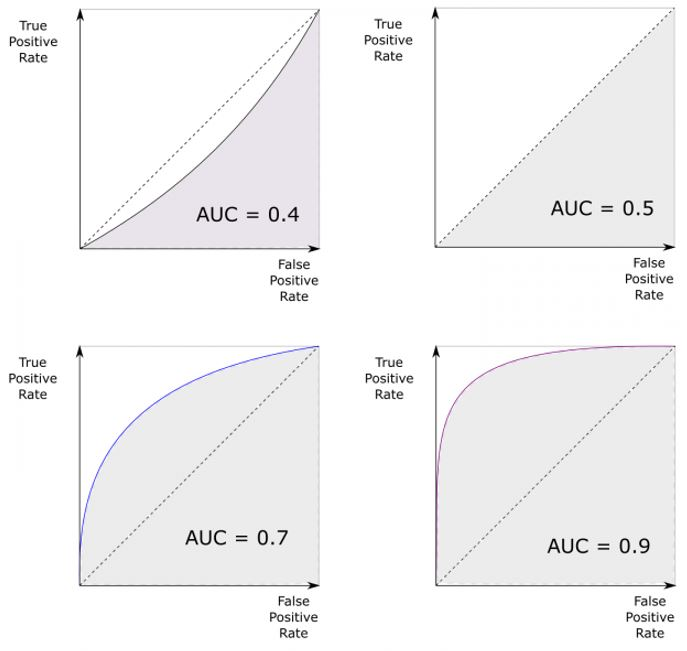
\includegraphics[scale = 0.5]{auc_1.JPG}
    \caption{แสดงความสัมพันธ์ของ AUC และ ROC Curve}
    \label{Fig:auc_0.4,5789}
\end{figure}

\subsection{Mean Average Precision (MAP)}
ในการแข่งขัน BirdCLEF 2020 นี้ทางผู้จัดแข่งขันได้เลือกใช้ metric ตัวนี้เป็นตัววัดและประเมินผลโดย MAP 
คือค่าเฉลี่ยของค่าความแม่นยำเฉลี่ย (Average Precision (AveP)) สามารถคำนวณได้จากสมการ~\ref{eq:MAP}

\begin{equation}
    MAP = \frac{\sum_{q=1}^{Q}AveP(q)}{Q}
    \label{eq:MAP}
\end{equation}

โดย Q คือจำนวนของไฟล์ที่ใช้ในการทดสอบแบบจำลอง และ Avep(q) 
สำหรับไฟล์ q ที่เป็นไฟล์ที่ใช้ในการทดสอบแต่ละไฟล์ซึ่งสามารถคำนวณได้ตามสมการ~\ref{eq:AveP}

\begin{equation}
    AveP = \frac{\sum_{k=1}^{n}(P(k)*rel(k))}{number\, of\, relevant\, document}
    \label{eq:AveP}
\end{equation}

